\section{Blog Challenge}\label{sec:blog-challenge}
\subsection{Challenge Overview}
%\todo[inline]{Provide a brief description of the challenge scenario, what participants need to accomplish (i.e., what skill is tested, the goal of the challenge).}
The "Exif Marks the Spot" challenge introduces players to OSINT\cite{WhatisOSINT} techniques through a simulated investigation. The players are presented with two websites: A fictional travel blog and a flight tracking platform. Their goal is to identify a specific return flight taken by a fictional professor by collecting information across both platforms. This challenge encourages reading, deduction, and technical skills such as metadata extraction and basic scripting, if needed. It is inspired by the common cybersecurity advice to avoid posting real-time vacation updates online, as such data can be exploited. Yannick was the primary developer of the challenge, from designing to implementing and testing, until the verification of the challenge itself, whereupon the group came up with ideas and encouragement to tweak upon the solve script.
\subsection{Technical Details}

%Step-by-step explanation of how the challenge works, including potential vulnerabilities, know how, or weaknesses that participants are expected to exploit. If possible use an image to illustrate the challenge architecture and how the different components interact.
\subsubsection{Design}
In the original challenge architecture, we had a lot of different features added to our websites, such as login forms, dynamic blog uploading, and live updating of flight schedules. However, as the project deadline approached, we decided to scrap these ideas and reallocate resources to other challenges. This resulted in the challenge architecture as visualized in Figure \ref{blog-architecture}, and consists of two separate front-end web applications hosted on different subdomains. One serves the blog content, and the other simulates a flight tracking service. Players are expected to navigate between the two, combining information to solve the challenge. We also use NGINX to split the traffic out onto the correct sites, based on the subdomain that the URL contains. Here we also have a healthcheck, ensuring that the CTF platform can check if the challenge is running. As shown in Figure \ref{blog-architecture}, the architecture consists of a few lightweight components that are implemented with the following tools and programming languages:
\begin{itemize} 
    \item \textbf{PHP} – for both the blog and flight tracker sites.
    \item \textbf{NGINX} - used as a reverse proxy to route HTTP traffic.
    \item \textbf{Docker} – for service isolation and portability.
    \item \textbf{Go} – used for the healthcheck service.
    \item \textbf{CSS} – for basic front-end styling.
\end{itemize}
\noindent
To speed up the development of the challenge, we also use ChatGPT for generating flight data and creating AI images, such as in Appendix \ref{fig:p12}. Another tool that was used for the challenge was ExifTool\cite{exiftool}, which was used for adding the metadata to the images, and also for extracting the data in the solve script to verify that the challenge is solvable.
\begin{figure}[H]
    \centering
    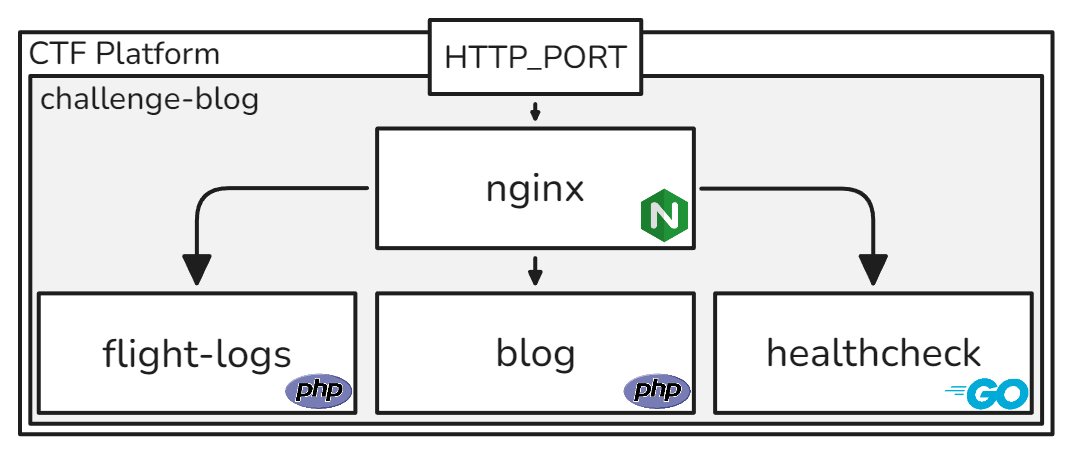
\includegraphics[width=0.8\linewidth]{img/challenge-blog--architecture.png}
    \caption{Blog challenge architecture}
    \label{blog-architecture}
\end{figure} 


\subsubsection{Challenge Flow and Solution}
The player is presented with two websites:
\begin{itemize}
    \item \texttt{https://blog.\$DOMAIN} – a personal travel blog
    \item \texttt{https://flight-logs.\$DOMAIN} – a simulated flight tracking service
\end{itemize}
Players start by exploring the blog, which belongs to “Professor PP.” They must read the posts, analyze image metadata, and take note of locations and dates. Most importantly, an image labeled \texttt{p12.png} (as shown in Appendix \ref{apx:p12}) contains EXIF metadata that reveals GPS coordinates and a timestamp, pointing to the professor's return flight date and departure location. EXIF is described more in section \ref{EXIF}. Using this information, the player then navigates to the flight tracking site and searches for flights that match the departure airport (NRT, Narita, Tokyo) and destination (CPH, Copenhagen), cross-referencing it with the date found. The solution to the challenge involves:
\begin{itemize}
    \item Visiting the blog site and parsing content.
    \item Downloading the image \texttt{p12.png}.
    \item Using \texttt{exiftool} to extract:
        \begin{itemize}
            \item GPS coordinates (indicating Narita, Japan)
            \item Date the photo was taken (2024-08-15)
        \end{itemize}
    \item Searching on the flight tracking site using the parameters:
        \begin{itemize}
            \item Departure: NRT
            \item Arrival: CPH
            \item Date: 2024-08-15
        \end{itemize}
    \item Extracting the correct flight number and generating the flag.
\end{itemize}
A solve script was created to automate this process using Bash\cite{Bash}, \texttt{curl}\cite{curl}, \texttt{wget}\cite{Wget}, \texttt{grep}\cite{grep}, \texttt{awk}\cite{Awk}, and \texttt{sed}\cite{Sed}, important snippets can be found in the appendix \ref{SolutionBlog} followed by the whole solution script. The final result is written to \texttt{/run/solution/flag.txt} as requested by the CTF platform standard.




\subsubsection{Difficulties Encountered}
%Describe any technical or conceptual challenges the group faced while creating this challenge.

% In the creation of the challenge itself, we didn't really face any difficulties, as we had thought a lot about the challenge beforehand and how to create it most efficiently before starting the development itself. But still, we wouldn't leave unharmed, as peril arose during the verification part of the challenge. Here we ran into trouble when trying to run the challenge on the CTF platform, as we had forgotten to use HTTPS instead of HTTP. This caused us trouble and drove us astray from completing the challenge. 

While the initial development of the challenge proceeded with minimal obstacles, some issues arose during the verification of the challenge on the CTF platform. These issues were not from the design or implementation of the challenge itself, but rather from how the CTF platform hosts websites. More specifically, the solvers' reliance on HTTP. The CTF platform enforced the use of HTTPS for interactions, a constraint that was initially overlooked during local testing, where HTTP had been enough. This discrepancy between the local and hosted environments resulted in communication failures between the solver script and the websites. Resolving this required a rewrite of the test script, resulting in two test scripts, one for local and one for the CTF platform. In the future, this could have been just a single script, checking the \texttt{\$DOMAIN} for the keyword local, and then differentiating on what it should accomplish. At the end, although ultimately resolved, this issue delayed the verification process and ended up taking time away from challenge hardening.
\subsubsection{Testing}
For this challenge, to ensure functionality, we created two different solve scripts, one for running in a local environment and one for running in a remote environment on the CTF challenge site. In the local environment, the website was hosted using HTTP. This allowed us to quickly identify errors and inconsistencies with our websites and solve scripts, without having to set up security. However, on the CTF platform, HTTPS is a requirement, meaning that a second solver script was established to mirror the secure conditions that the platform enforces and under which the challenge ultimately would be verified. The testing itself involved both a manual verification, meaning we as a group have manually completed the challenge, navigating the websites and gathering information, to create the finished flag. But an automated script for validation was also created. The script \texttt{solver.sh} is an automated Bash script for solving the challenge. The script replicates the players' expected journey, beginning with the retrieval of the starting IATA code, followed by the blog's image acquisition, extraction of EXIF metadata on said blog, and ending with a search query on the simulated flight tracker website. The script then verifies the flag by writing the result to \texttt{/run/solution/flag.txt} path, as dictated by the CTF platform. Some of the code snippets can be found in the Appendix \ref{SolutionBlog}. After having locally validated the challenge, it was then deployed to the CTF platform and verified successfully with the challenge ID: \texttt{77847818-6c37-4dc9-ad1d-8a63b1ba3e9c}


\subsubsection{EXIF}\label{EXIF}
Exchangeable Image File Format is a file format typically used for storing data about pictures. The EXIF metadata is automatically embedded into image files. This constitutes as the main security vulnerability in the Blog Challenge, as the pictures aren't sanitized, making it possible to find information from advanced cameras.
Listing \ref{lst: exiftoolusedonp12} demonstrates the output of \texttt{exiftool} being run on the file \texttt{p12.png}. 
% As shown, important fields such as Date/Time Original, and GPS Position is appearing.
\begin{listing}[H]
  \begin{minted}[linenos]{javascript}
ExifTool Version Number         : 12.40
File Name                       : p12.png
Directory                       : .
File Size                       : 1542 KiB
File Modification Date/Time     : 2025:05:21 14:03:15+02:00
File Access Date/Time           : 2025:05:25 14:21:43+02:00
File Inode Change Date/Time     : 2025:05:21 14:03:15+02:00
File Permissions                : -rwxr-xr-x
File Type                       : PNG
File Type Extension             : png
Date/Time Original              : 2024:08:05 20:10:37
GPS Version ID                  : 2.3.0.0
GPS Latitude                    : 35 deg 46' 9.38"
GPS Longitude                   : 140 deg 23' 23.63"
Image Size                      : 1024x1024
Megapixels                      : 1.0
GPS Position                    : 35 deg 46' 9.38", 140 deg 23' 23.63"
  \end{minted}
  \vspace{-1.5\baselineskip} % Justerer afstanden mellem tekst og liste
 \caption{Exiftool used on p12.png (Shown in Appendix \ref{fig:p12})}
\label{lst: exiftoolusedonp12}
\end{listing}

\subsubsection{Difficulty Assessment}
%Rate and justify the challenge’s difficulty level.
This challenge was intentionally designed to be easy, serving as an accessible entry point for CTF newcomers and an entry point into OSINT. Its purpose was to introduce and engage beginners with minimal prior experience in cybersecurity, while still reinforcing and introducing them to topics such as metadata analysis and cyber hygiene. The required tools, such as \texttt{curl}, \texttt{grep}, and \texttt{exiftool}, if your approach is terminal-based, are widely known and documented, making it straightforward to use and approachable. The challenge could also be completed using purely visual tools, by manually downloading the images and extracting their metadata through websites such as \href{https://exif.tools/}{exif.tools}. While we consider the difficulty of the challenge to be easy, it still introduces important concepts such as cyber hygiene and metadata analysis. As such, the challenge works as intended, gathering attraction to CTFs by both being educational and approachable. 


% \subsubsection{Improvements}
% While the challenge met its intended goals, some improvements could be made to enhance the player experience and the technical depth.
% Instead of hardcoding the EXIF data, we could have dynamically generated the metadata using scripts on challenge starts, which could have increased reusability. So instead of having a hardcoded date of summer 2024. It could have been made so it was in response to when the player is playing the challenge, such as June 2025. This could also reduce walkthrough reuse, so other players couldn't just get the answer from another source.
% In general, the front-end design was also kept minimal. This could have been changed to have a better aesthetic or better uphold Jakob Nielsen's 10 Heuristics.
% Another thing we could have worked more upon would be to add more layers of OSINT that the player should have had to go through, which in turn would deepen the educational value that the players would have gotten, such as playing around with social media profiles or experimenting with steganography.
% But overall, we believe that the challenge lays a strong foundation for a beginner-friendly OSINT task, but with some additional refinements, it could evolve into a more robust and scalable learning experience. 